\documentclass[
  ngerman,
  color=8c,
  submission,
  boxarc,
  fleqn,
]{rubos-tuda-template}

\usepackage{drawstack}
\usepackage{pgfplots}
\usepackage{tabularray}
\usepackage{numberedblock}

\groupnumber{3}
\addSubmittor{Bora Büyükbas}{}
\addSubmittor{Philip Seitz}{}
\addSubmittor{Fares Elkholy}{}
\groupLeader{<Gruppenleitername>}
\semester{SoSe 2024}
%\version{1.0}
\fachbereich{Informatik}
% \dozent{<Prof>}
\date{\today}
\termStyle{left-right-manual}
\termLeft{%
    printAuthor,%
    printSubmittors,%
}
\termRight{%
    printSheetNumber,%
    %printVersion,%
    printGroupNumber,%
    %printGroupLeader,%
    printSemester,%
}

\begin{document}

\title[Parallele Programmierung]{Performance Analysis für Aufgabe 5b\\ Parallele Programmierung}

\maketitle{}
\textbf{Hinweis:} Alle Tests wurden im Lichtenberg-Hochleistungsrechner fünfmal für jeden Wert durchgeführt, und die Durchschnittswerte dieser Tests sind in den Grafiken dargestellt.

\section{Rechenintensive Teile der Methode}
Um einen vernünfitgen Speed up zu erreichen, haben wir zwei parallele Regionen in unserer Methode eingefügt. 
% Erläutern Sie, welche Teile der Methode Sie als besonders Rechenintensiv ansehen und warum.

Einmal haben wir die verschachtelte for-Schleife (beginnend auf Zeile 57 in \verb|find_collisions()|) parallelisiert. Diese wird dafür verwendet, potenziel kollielierende Paare von Körper zu finden. Für jeden arbeitenden Thread ist dann eine \verb|private_pair_set| vorgesehen, in der die gefundenen Paare gespeichert werden. Am Ende der parallelisierten for-Schleife werden die Ergebnisse der jeweiligen Threads in die \verb|pair_set| zusammengeführt. Wir haben diese for-Schleife parallelisert, da sie bei $10^5$ Körper insgesamt $(10^5)^2 = 10^{10}$ Iterationen durchführt und somit sehr rechenintensiv ist. Wie unten zu sehen ist, ist dieser Teil der Methode tatsächlich das am rechenintensivsten. 
Zuletzt haben wir die für das Löschen der kollidierte Körper zuständige for-Schleife (beginnend auf Zeile 101) parallelisert. Da die Anzahl der Körper, die gelöscht werden müssen, in der Regel deutlich geringer ist als die Anzahl der Körper, die auf Kollisionen überprüft werden müssen, ist dieser Teil der Methode viel weniger rechenintensiv. Dennoch haben wir ihn parallelisiert, um den Speed up zu maximieren. \newline

% Belegen Sie Ihre Vermutungen durch geeignete Messungen
Um die Rechenintensivität dieser zwei Teile der Methode zu belegen, haben wir die Laufzeit der Methode für verschiedene Anzahlen von Körpern gemessen, wobei alle anderen Teile der Methode nicht geändert wurden. Die folgende Grafik zeigt die Laufzeit der Methode für $10^2$ bis $10^7$ Körper. Die Laufzeit der Methode steigt exponentiell mit der Anzahl der Körper. 
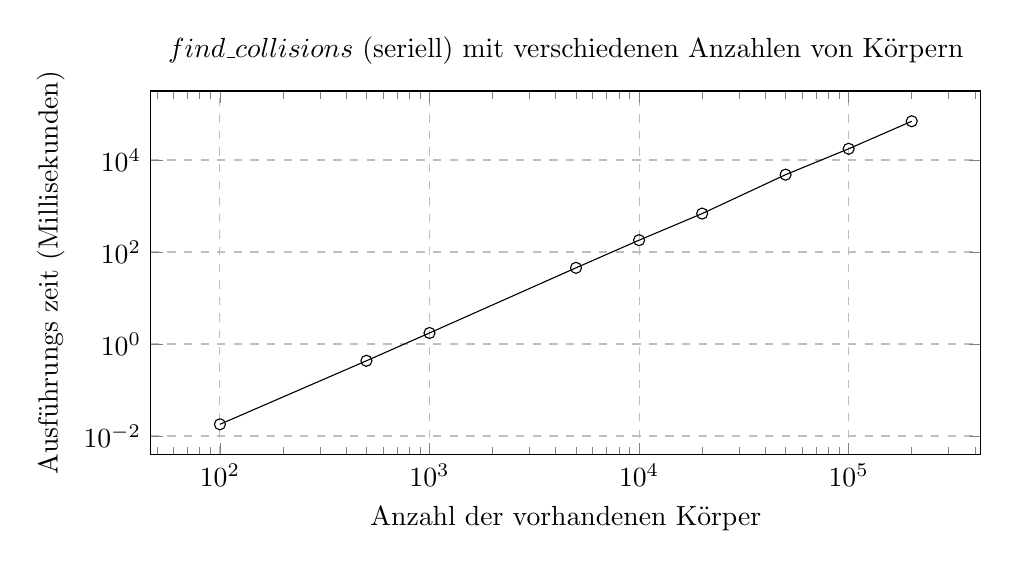
\begin{tikzpicture}
    \begin{axis}[
        title={$find\_collisions$ (seriell) mit verschiedenen Anzahlen von Körpern},
        ymode=log,
        xmode=log,
        width=\textwidth,
        height=6.2cm,
        xlabel={Anzahl der vorhandenen Körper},
        ylabel={Ausführungs zeit (Millisekunden)},
        log basis y={10},
        grid=major,
        grid style=dashed,
      ]
        \addplot[mark=o] coordinates {
          (100, 0.018)
          (500, 0.432)
          (1000, 1.74)
          (5000, 45.3)
          (10000, 181)
          (20000, 685)
          (50000, 4804)
          (100000, 17559)
          (200000, 69626)
        };
      \end{axis}
\end{tikzpicture}

Die Messungen zeigen, dass die Ausführungszeit besonders ab etwa 5.000 Körpern deutlich zunimmt.
Weil diese zwei Teile der Methode stark von der Anzahl der Körper abhängig sind, zeigen diese Messungen auch, dass mit einer ansteigenden Anzahl von Körper diese Teile der Methode sehr rechenintensiv werden und daher eine Parallelisierung sinnvoll ist.

\section{Effektivität der Parallelisierung durch OpenMP}
% Zeigen Sie zudem die Effektivität ihrer Parallelisierung anhand geeigneter Messungen und dem Vergleich mit find_collisions.

% 1: plot graph of speedup on y-axis and number of bodies on x axis


Um die Effektivität der Parallelisierung zu zeigen, haben wir die Laufzeit der beiden Methoden für verschiedene Anzahlen von Körpern gemessen. 

Die folgende Grafik zeigt den jeweiligen Unterschied der Ausführungszeiten der Methode für verschiedene Anzahlen an Körper zwischen $10^2$ bis $10^5$.

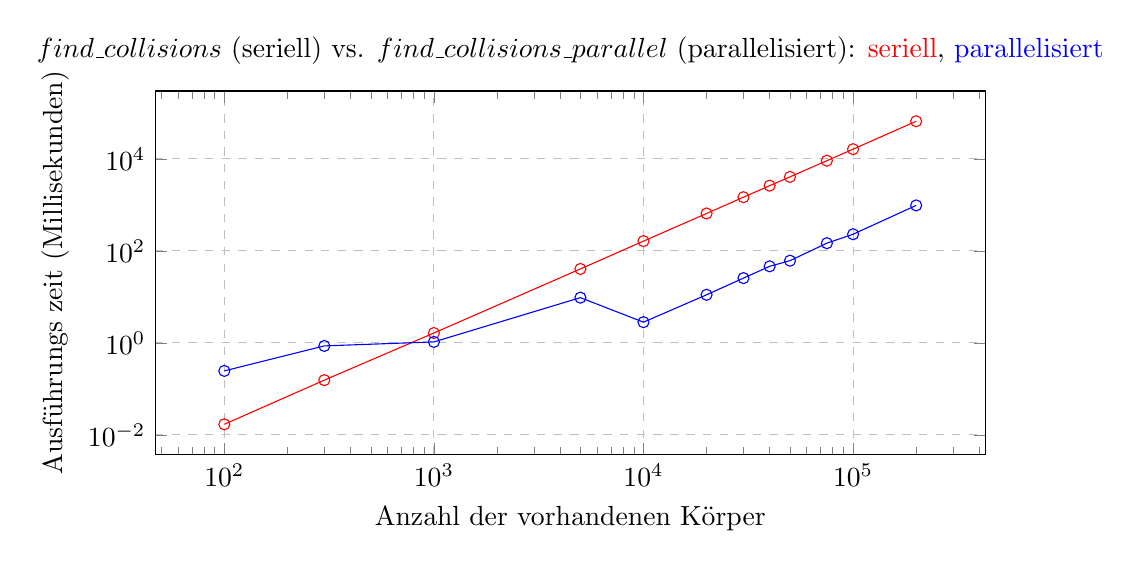
\begin{tikzpicture}
  \begin{axis}[
      width=\textwidth,
      height=7cm,
      title={$find\_collisions$ (seriell) vs. $find\_collisions\_parallel$ (parallelisiert): \textcolor{red}{seriell}, \textcolor{blue}{parallelisiert}},
      ymode=log,
      xmode=log,
      width=\textwidth,
      height=6.2cm,
      xlabel={Anzahl der vorhandenen Körper},
      ylabel={Ausführungs zeit (Millisekunden)},
      log basis y={10},
      grid=major,
      grid style=dashed,
    ]

    \addplot[
      color=red,
      mark=o,
    ]
    coordinates {
        (100, 0.017)
        (300, 0.155)
        (1000, 1.64)
        (5000, 40.5)
        (10000, 163)
        (20000, 650)
        (30000, 1469)
        (40000, 2616)
        (50000, 4056)
        (75000, 9140)
        (100000, 16235)
        (200000, 65735)
      };

    \addplot[
      color=blue,
      mark=o,
    ]
    coordinates {
        (100, 0.246)
        (300, 0.860)
        (1000, 1.05)
        (5000, 9.63)
        (10000, 2.82)
        (20000, 11.1)
        (30000, 25.6)
        (40000, 46.2)
        (50000, 61.2)
        (75000, 147)
        (100000, 230)
        (200000, 974)
      };
  \end{axis}
\end{tikzpicture}

Das Diagramm zeigt, dass zwar die paralleliserte Methode für kleine Anzahlen von Körpern (ca. $10^2$ Körper) langsamer ist als die serielle Methode, jedoch für größere Anzahlen von Körpern deutlich schneller ist. Dies ist darauf zurückzuführen, dass die serielle Methode für große Anzahlen von Körpern sehr rechenintensiv ist und die parallelisierte Methode die Rechenlast auf mehrere Threads verteilt.

Zum Beispiel wurde es für eine Körperanzahl von 100000 einen 50x-Speedup der Ausführungszeit der paralleliserten Methode im Vergleich zur serillen erreicht. Damit lässt sich abschließend behaupten, dass die Parallelisierung der Methode (für die meisten Fälle) sehr effektiv ist.

\end{document}
